\documentclass[a4paper,11pt]{article}

\usepackage{multicol}
\usepackage{verbatim}
\usepackage{enumerate}
\usepackage{enumerate}

\usepackage{fancyvrb}

\usepackage{graphicx}
\usepackage{color}
\usepackage{subfigure}
%\usepackage{epsfig}
\usepackage{xspace}

\usepackage[latin1]{inputenc}
\usepackage[T1]{fontenc}
\usepackage{pslatex}
\usepackage[english]{babel}

\usepackage[colorlinks=true,linkcolor=black]{hyperref}

%%%%%%%%%%%%%%%%%%%%%%%%%%%%%%%%%%
%%%%%  reviewer comments  %%%%%%%%
%%%%%%%%%%%%%%%%%%%%%%%%%%%%%%%%%%
\newcommand{\comm}[2]{{\sf \(\spadesuit\){\bf #1: }{\rm \sf #2}\(\spadesuit\)}}
\newcommand{\mcomm}[2]{\marginpar{\scriptsize \comm{#1}{#2}}}
%\renewcommand{\comm}[2]{}
%%%%%%%%%%%%%%%%%%%%%%%%%%%%%%%%%%
\newcommand{\jbcomment}[1]{\mcomm{JB}{#1}}
\newcommand{\cocomment}[1]{\mcomm{CO}{#1}}

% Fancy code with color commands:
\DefineVerbatimEnvironment{fancycode}%
        {Verbatim}{commandchars=\\\{\}}

%%%%%%%%%% The language %%%%%%%%%%
\newcommand{\fasto}{\textsc{Fasto}\xspace}
\newcommand{\mips}{\textsc{Mips}\xspace}
\newcommand{\mars}{Mars\xspace}

\title{A Compiler for The \fasto Language}

\author{Group Project for the Compiler Course}

\date{Block~2, Winter 2012/13}

\begin{document}

%\setlength{\baselineskip}{0.95\baselineskip}

\maketitle

\tableofcontents

\section{Introduction}

This is the description of the project for the Compilers Course (Overs\ae{}ttere), 
in  block 2 of 2012-2013.
%
The project should be solved in groups of (up to) three students.
%
The task is available from Monday, Nov.19, 2012 (after the lecture), 
and solutions must be handed in by 
Friday, Dec.21, 2012 (2:00pm), by uploading code and report via the course website at Absalon.
Use the group submission function in Absalon, and indicate the names of all 
group members in the report. There is no standard format, please create one yourselves.

This project will be assessed as passed or failed, without a mark.
Approval of this task is a prerequisite for participation in the 
final exam (in addition to approval of at least four of the five
weekly assignments), and \emph{cannot be resubmitted}.
%
%The exam task is be solved individually. 



\section{Project / Task Description}

\subsection{Overview}
The task is to implement a compiler for the \fasto
language\footnote{\fasto stands for "Funktionelt Array-Sprog Til Overs\ae{}ttelse".},
described in detail in Section~\ref{fasto}.
In summary, \fasto is a simple strongly-typed first-order functional
language which supports
arrays by special array constructors and combinators 
(\texttt{map} and \texttt{reduce}).

You are not required to implement the whole compiler from scratch:
We provide a partial implementation of \fasto, 
and you are asked to add the missing parts to produce a working
implementation of the entire language.
%
The partial implementation, as well as a number of input programs 
and expected output for tests, can be found in the archive \emph{Fasto.zip}.
%\jbcomment{OLD! If we plan to add stuff, we should say 'will', not 'may'}
%Additional input programs may be handed in within two weeks of the start
%date of the project.  
The archive contains four subfolders: 
\begin{description}
\setlength{\itemsep}{0.1ex}

\item[{\tt SRC/}:] contains the implementation of the compiler.

\item[{\tt DATA/}:] contains test inputs and expected output files.

\item[{\tt DOC/}:] contains documentation, e.g., this document and {\tt mips-module.pdf}.

\item[{\tt BIN/}:] will contain the compiler executable (binary) file.

\end{description}

To complete the task you will need to modify the following files in {\tt SRC} folder:
 
\begin{description}
\setlength{\itemsep}{0.1ex}

\item[{\tt Lexer.lex}:] Lexical definition of \fasto's tokens, to be used with \texttt{mosmllex}. 

\item[{\tt Parser.grm}:] The implementation of \fasto's grammar, 
	to be used with \texttt{mosmlyac}. 
	The parse result is the abstract syntax tree of the input program.

\item[{\tt Fasto.sml}:] The abstract syntax of \fasto, 
       and functions to format and print entities of a \fasto program.

\item[{\tt Interpret.sml}:] An interpreter for \fasto.

\item[{\tt Type.sml}:] Type-checker for \fasto.

\item[{\tt Optimization.sml}] High-level optimizations for \fasto.

\item[{\tt Compiler.sml}:] Translator from \fasto to \mips assembler.
    The translation is done directly from \fasto to \mips, i.e., without 
        passing through a lower-level intermediate representation of the code.

\end{description}

\noindent
There are two more modules in the compiler: a register allocator
(\texttt{RegAlloc.sml}), and functions and types for \mips instructions
(\texttt{Mips.sml}).  Most likely it will not be necessary to modify these
files.

The main program {\tt FastoC.sml} is the driver of the compiler: it runs the 
lexer and parser, and then either interprets the program or
validates the abstract syntax in the type checker, rearranges it in 
the optimizer, and compiles it to \mips
code. After the type checker validates the program, the other stages assume
that the program is type-correct. (Some type information needs to be retained
for code generation, and is added by the type checker when unknown.)
To run the interpreter on a file located at \texttt{DATA/file.fo}, use option ``-i'', 
{\tt\$BIN/FastoC -i DATA/file} (omit the file extension {\tt .fo}). To compile the
file with optimizations, use option ``-o''. Otherwise use no option,
i.e.,   {\tt\$BIN/FastoC DATA/file}.

{\em The compiler modules are described in detail in Appendix~\ref{sec:modules}.}

Please use the Moscow ML~\cite{MoscowML} compiler, {\tt mosmlc}, to compile the 
above modules, including the unchanged ones. For lexical and syntactical
analysis, please use Moscow ML's tools {\tt mosmllex} and {\tt mosmlyac}.
(We have tested our implementation and will evaluate yours with these tools.)
%
Files {\tt SRC/compile.sh} and {\tt SRC/compile.bat} contain commands
to rebuild all modules and the compiler under Linux and Windows, respectively.
Some of the modules might generate compiler warnings, which can be
safely ignored, but please be aware of any new error messages or warnings introduced
by your changes to the code, i.e., check that the newly introduced warnings are indeed 
harmless and not bugs in your code.
The bundle also contains makefiles, but you are not required to understand or 
use them.

To run the programs compiled by the compiler, you should use the \mars
simulator~\cite{Mars}. \mars is written in Java, so you need a Java Runtime
Environment in order to use it. There is a link to \mars from the course
Absalon page, also see the short description in \texttt{DOC/mips-module.pdf}.

\subsection{Features to Implement}
In brief, you need to implement the 
following features in the assignment:

\begin{itemize}
\setlength{\itemsep}{0.1ex}

\item multiplication, division, boolean operators 
(\textsc{and}, \textsc{or}, \textsc{not}), boolean literals;
%
\item bounds-checking for array indexing;
%
\item using operators as functions in array combinators
(explained in \ref{subsec:map-red-prog});
%
\item one of the array combinators \texttt{zipWith} or 
\texttt{scan}, explained in \ref{subsec:map-red-prog}, 
and either a \texttt{length} function or a \emph{polymorphic} 
\texttt{write} function;
\item an optimization pass to eliminate unused functions.
\end{itemize}
The project tasks are described in detail in Section~\ref{sec:Tasks}, after the 
language description.

\noindent
Your solution should demonstrate competence in the entire curriculum,
understanding of all compiler phases and the ability to thoroughly document your
solution. 
%
Partial solutions will be considered if they are convincing and well-documented.

\subsection*{Submitting Your Solution}

A solution to this assignment consists of two files to be uploaded to Absalon:
\begin{enumerate}
\item A \texttt{zip} or \texttt{tar.gz} archive containing the full implementation 
	of the compiler and tests. Please use the same directory structure as 
	\emph{Fasto.zip} (source code in \texttt{SRC}, tests in \texttt{DATA}).
	Do not submit any binaries, but make sure that the script 
	\texttt{compile.[bat|sh]} still works and produces your compiler as {\tt BIN/FastoC}.
\item a written \emph{report} describing and evaluating your work and the main design 
	decisions you took. %in your implementation. 
	The report should not exceed 16 pages of text, and must start by a 
	cover page which states all group members by name.
\end{enumerate} 

Files are delivered via the course website. Use the group submission
feature of Absalon, i.e., submit only one copy per group.

\paragraph{Contents of the Report}
The report shall include justification of the changes that
were made in every compiler stage, i.e., lexer, parser, interpreter,
type checker, machine-code generator.

When evaluating your work, the main focus will be to verify that the
implementation of the language is {\em correct}.  While we do not
put particular emphasis on compiler optimizations in this course, 
we will also evaluate the {\em quality of the generated code}: 
if there are obvious inefficiencies that could have been easily 
solved you will be penalized, as they testify either wrong priorities 
or lack of understanding.

You should not include the whole compiler code in the content
of your report, but you {\em must} include the parts that were either
added, i.e., new code, or substantially changed.  Add them as
Figures, or code listings in Annexes or the like.   
%
If you refer to implementation code, this must also be included
in the report document.

The report shall describe whether the compilation and execution of
your input/test (\fasto) programs results
in the correct/expected behavior. If it does not, it should explain how 
and why it deviates from the expected behavior. In addition, (i) it must 
be assessed to what extent the delivered test programs cover all
programming patterns, and (ii) if the implementation deviates from the 
expected behavior then the test program(s) should illustrate the %implementation 
shortcoming to its largest extent. 

Known shortcomings in type checking and compilation must be described, 
and, whenever possible, you need to make suggestions on how these might
be corrected.
%
It is largely up to you to decide what you think is important to include 
in the report, as long as the explicit requirements of this section are met.

The report should be kept below 16 pages, and it should include all 
important information: all major design decisions should be presented 
and justified, and all deficiencies must be described.   Ideally, we
should not need to read your source code.
You might be penalized if your report includes too many irrelevant details. 

\subsection{Accepted Limitations of the Compiler}

It is perfectly acceptable that the lexer, parser, type checker and code 
generator stops at the first error encountered.

It can be assumed that the translated program is small, so all target addresses 
for jump and branch instructions fit into constant fields of \mips jump instructions.
(i.e. label addresses fit into 16 bit, for branch instructions).

It is not necessary to free memory in the heap while running the program.
You do not need to consider stack or heap overflow in your implementation. 
The actual behavior of overflow is undefined, so if errors occur during execution,
or you see strange results, it might be due to overflow.




\subsection{MosML-Lex and MosML-yacc}

Documentation related to these tools is available in Moscow ML Owners Manual.
The manual can be found on the Moscow ML homepage~\cite{MoscowML}, which 
also provides installation information for Windows and Linux. 
The course website contains a direct link to the manual, and also provides
an independent example of using Moscow ML's lex and yacc tools 
({\tt Lex+Parse.zip}), in Danish. 

\section{The \fasto Language\label{fasto}}
\fasto is a simple, first-order-functional language that allows
recursive definitions. In addition to simple types (\texttt{int, bool, char}),
\fasto supports arrays, which can also be nested, by providing array constructor
functions (\textsc{ac}s) and second-order array combinators (\textsc{soac}s)
to modify and collapse arrays.
%
Before we give details on the array constructors and combinators,
we present the syntax and an informal semantics of \fasto's basic constructs.

\newcommand{\keyw}[1]{\mbox{\texttt{#1}}}
\newcommand{\tok}[1]{\mbox{\sc #1}}
\begin{figure}[t!]
% two-column layout for grammar
\renewcommand{\arraystretch}{0.87}
\begin{minipage}{0.5\textwidth}
\[
\begin{array}{lcl}
Prog & \rightarrow & FunDecs \\[0.9ex]

FunDecs & \rightarrow & \keyw{fun} \ Fun \ FunDecs \\
FunDecs & \rightarrow & \keyw{fun} \ Fun \\
Fun & \rightarrow & Type \ \tok{ID} \ ( TypeIds ) = \ Exp  \\
Fun & \rightarrow & Type \ \tok{ID} \ ( ) = \ Exp  \\[0.9ex]

TypeIds & \rightarrow & Type \ \tok{ID}\ ,\ TypeIds\\
TypeIds & \rightarrow & Type \ \tok{ID}\\[0.9ex]

Type & \rightarrow & \keyw{int} \\
Type & \rightarrow & \keyw{char} \\
Type & \rightarrow & \keyw{bool} \\
Type & \rightarrow & [ \ Type \ ] \\ [0.9ex]

Exp & \rightarrow & \tok{ID} \\
Exp & \rightarrow & \tok{NUM} \\
Exp & \rightarrow & \tok{CHARLIT} \\
Exp & \rightarrow & \tok{STRINGLIT} \\
Exp & \rightarrow & \{ \ Exps\ \}\\
\end{array}
\]
\hspace*{2em}\textit{(\ldots continued on the right)}
\end{minipage}\hspace*{2em}
\begin{minipage}{0.5\textwidth}
\[
\begin{array}{lcl}
Exp & \rightarrow & Exp \ \tok{+} \ Exp \\
Exp & \rightarrow & Exp \ \tok{-} \ Exp \\
Exp & \rightarrow & Exp \ \tok{=}\ Exp \\
Exp & \rightarrow & Exp \ \tok{<} \ Exp \\
Exp & \rightarrow & ( \ Exp \  )\\
Exp & \rightarrow &  \keyw{if}\ Exp\ \keyw{then}\ Exp\ \keyw{else}\ Exp \\
Exp & \rightarrow & \keyw{let} \  \tok{ID} \ = \ Exp \ \keyw{in} \ Exp\\
Exp & \rightarrow & \tok{ID} \ ( \ Exps \  )\\
Exp & \rightarrow & \tok{ID} \ (\ ) \\
Exp & \rightarrow & \keyw{read} \ ( \ Type \ )\\
Exp & \rightarrow & \keyw{write} \ ( \ Exp \ )\\[0.9ex]
Exp & \rightarrow & \tok{ID} \ [ \ Exp \ ]\\
Exp & \rightarrow & \keyw{iota} \ ( \ Exp \ )\\
Exp & \rightarrow & \keyw{replicate} \ ( \ Exp \ , \ Exp \  )\\
Exp & \rightarrow & \keyw{map} \ ( \ \tok{ID} \ , \ Exp \ )\\
Exp & \rightarrow & \keyw{reduce} \ ( \ \tok{ID} \ , \ Exp \ , \ Exp \ )\\[0.9ex]

Exps & \rightarrow & Exp \ , \ Exps\\
Exps & \rightarrow & Exp \\

\end{array}
\]
\end{minipage}
\renewcommand{\arraystretch}{1.0}
\caption{Syntax of the \fasto Language.}
\label{fig:FastoGram1}
\end{figure}

\subsection{Lexical and Syntactical Details}
\label{subsec:lexicalrules}
A context-free grammar of \fasto is given in Fig.~\ref{fig:FastoGram1}.
The following rules characterise the \fasto lexical atoms and clarify the syntax.

\begin{itemize}
\item A name ({\bf ID}) consists of (i) letters, both uppercase and lowercase,
   (ii) digits and (iii) underscores, but it {\em must} begin with a letter. 
   Letters are considered to range from $A$ to $Z$ and from $a$ to $z$, i.e., 
   English letters. 
   %
   Some words ({\tt if, then, fun,}\ldots) are reserved keywords and {\em cannot} 
   be used as names.
  
\item Numeric constants, denoted by {\bf NUM}, take positive values, and 
   are formed from digits $0$ to $9$. Numeric constants are limited to 
   numbers that can be represented as positive integers in Moscow ML.
%
  A possible minus sign is \emph{not} considered as part of the number literal
  (negative number literals are not supported in the handed-out version, one would 
  need to write {\tt 0-1} for {\tt -1}).

\item A character literal ({\bf CHARLIT}) is surrounded by single quotes 
   (\texttt {'}). A character literal is:
  \begin{enumerate}
  \item A character with ASCII code between $32$ and $126$ \emph{except}
     for characters \texttt{\underline'}, \texttt {\underline"} and \underline{\textbackslash}.
  \item An \emph{escape sequence}, consisting of character 
  \underline\textbackslash, 
  followed by one of the following characters: 
  \texttt{a, b, f, n, r, t, v, ?, \underline', \underline"}, or
  by an octal value between 0 and 0177, 	or by \texttt{x} and a 
  hexadecimal value between 0 and 0x7f.
  \end{enumerate}

\item A string literal ({\bf STRINGLIT}) consists of a sequence of
   characters surrounded by double quotes (\texttt {"}).
	Escape sequences as described above can be used in string literals.
  
\item The {\tt +} and {\tt -} operators have the same precedence and
   are both left-associative.

\item The {\tt <} and {\tt =} operators have the same precedence and 
   are both left-associative, but they both bind weaker than {\tt +}.

%\item The assignment operator, also denoted by {\tt =}, binds weaker than {\tt <} and is
%   right-associative.

%\item {\tt else} binds to the nearest \texttt{if} as described in the textbook.

%\item Variables and functions live in separate namespaces.

\item Any sequence of characters starting with {\tt //} and ending at the 
	end of the respective line is a comment and will be ignored by the parser.

  \item Whitespace is irrelevant for \fasto, and no lexical atoms 
  	contain whitespace.

\end{itemize}

\subsection{Semantics}

\fasto implements a small functional language;
unless otherwise indicated, the language semantics is similar to 
that of {\sc sml}.  With the exception of IO read and write 
operations this subset is pure, e.g., no destructive updates.

\subsubsection{\fasto Basics}

As can be seen in Fig.~\ref{fig:FastoGram1},
a \fasto program is a list of function declarations.

\noindent
Any program must contain a function called \texttt{main} that does
not take any parameters.
The execution of a program always starts with/calls the 
{\tt main} function. Function scope spans through the entire 
program, so any function can call  another one and, for instance, 
functions can be mutually recursive without special syntax. It is illegal
to declare two functions with the same name.   

Each function declares its result type and the types and names of
its formal parameters. It is illegal for two parameters
of the same function to share the same name. Functions and variables
live in separate namespaces, so a function can have the same name as a 
variable. The body
of a function is an expression, which can be a constant (for instance {\tt 5}),
a variable name ({\tt x}), an arithmetic expression or a comparison ({\tt a<b}), 
a conditional ({\tt if e1 then e2 else e3}), a function call ({\tt f(1,2,3)}), 
an expression with local declarations, ({\tt let x = 5 in x + y}), and so on.   

 
\subsubsection{\fasto Built-In Functions}
\label{subsec:built-ins}

Since \fasto is strongly typed and does not support implicit casting, built-in
functions ${\tt{}chr} : {\tt{}int} \rightarrow {\tt{}char}$ and 
${\tt{}ord} : {\tt{}char} \rightarrow {\tt{}int}$ 
allow one to convert explicitly between integer and character values. 
They are represented internally as ``regular' functions, because their
types are expressible in \fasto, i.e., not polymorphic.

Function {\tt read} and {\tt write}, which read and write to standard input
and output, are the only \fasto constructs having side effects ({\sc io}); 
the language is otherwise {\em purely functional}.
Since {\tt read} and {\tt write} are polymorphic (and their types not expressible in \fasto),
the parser does not treat calls to them as function calls,
but instead represents them by special {\tt Read} and 
{\tt Write} nodes in the abstract syntax.

{\tt read} receives a type parameter that indicates the type of the value to be read:
{\tt read(int)} returns \texttt{int}, {\tt read(char)} and {\tt read(bool)} return 
\texttt{char} and \texttt{bool}, respectively. These are all the valid uses of {\tt read}.

{\tt write} outputs the value of its parameter expression, and returns this value.
Its valid argument types are {\tt int}, {\tt char}, {\tt bool}, and {\tt [char]} 
(the type of string literals and arrays of characters), 
e.g., {\tt write("Hello World!")}. 



%\fasto provides several built-in functions:
%
%\begin{itemize}
%    \item {\tt chr : int $\rightarrow$ char} converts an integer to a character value.
%    \item {\tt ord : char $\rightarrow$ int} converts a character to an integer value.
%    \item {\tt read(int)}, {\tt read(bool)} or {\tt read(char)} read from standard input 
%            an integer, boolean, or character value, respectively.
%    \item {\tt write} to standard output an expression of type {\tt int}, {\tt char}, 
%            {\tt bool}, or {\tt [char]}.
%\end{itemize}



\subsubsection{(Multidimensional) Arrays in \fasto}


\fasto supports three basic types: {\tt int}, {\tt char} and {\tt bool}.
Comparisons are defined on values of all basic types, but addition, 
subtraction and the like are {\em only} defined on integers.
As a rule, % JB: YES! ;-)
no automatic conversion between types is carried out, e.g.,
{\tt let a = if(cond) then 'c' else 1}
should be rejected by the type checker.

{\em In addition}, \fasto supports an array type constructor, 
denoted by {\tt []}. Arrays can be nested. 
For example, type {\tt [char]} denotes the type of a
vector of characters,  {\tt [[int]]} denotes the type of a two-dimensional 
array of integers, {\tt [[[bool]]]} denotes the type of a
three-dimensional array of booleans, etc.  
%
Single-dimension indexing can be applied on arrays: if {\tt x :{}[[int]]},
then {\tt x[0]} yields the first element of array {\tt x}, and
{\tt x[i]} yields the {\tt i+1} element of {\tt x}. Both {\tt x[0]} and {\tt x[i]}
are arrays of integers, i.e., have type {\tt [int]}. If the index is outside
the array bounds, the result is undefined (but you will fix this!)
%
Arrays can be built in several ways: % in \fasto:
\begin{itemize}
    \item By the use of arrays literals, as exemplified in the following expression:\\
        {\tt let x = 1 in \{ \{1+x, 2+5\}, \{3-x, 4, 5\} \}}.\\
        This represents a bi-dimensional arrays of integers, 
        thus type {\tt [[int]]}.\\
        Note that array elements can be arbitrary expressions, 
        not just constants.
    \item String literals are supported and they are identical to one-dimensional
            arrays of characters, i.e., {\tt "abcd" } is the same
            as {\tt \{ 'a', 'b', 'c', 'd' \}}.\\ 
            Both arrays of characters and string literals are stored with 
            an extra null {\tt 0} character at the end, which allows the 
            {\sc io}-system calls of \mips to use them.
    \item {\tt iota} and {\tt replicate} are array constructors ({\sc ac}):
            {\tt iota(N)}$\equiv${\tt \{0,1,..,N-1\}}, i.e., it constructs the
            uni-dimensional array containing the first $N$ natural integers 
            starting with $0$.
            Note that $N$ can be an arbitrary expression of integer type, and 
                that the result is always of type {\tt [int]}.
    \item Similarly, {\tt replicate(N, val)}$\equiv${\tt \{val, val, .., val\}},
            creates an array of {\tt N} elements (hence {\tt N}
            needs to be of type {\tt int}), filled with the given
            element {\tt val} as a constant.
          The result array has the element type of {\tt val}, and
            adds an extra-dimension to those of {\tt val}, e.g.,
            if the type of {\tt val} is {\tt [[bool]]}, then the result is a 
            $3D$ array of booleans, i.e., {\tt [[[bool]]]}.  
\end{itemize}



\subsubsection{Map-Reduce Programming with \fasto Arrays}
\label{subsec:map-red-prog}

We have seen so far how arrays are constructed from a (finite) set of
literals, from a scalar (with {\tt iota}), or by copying (with \texttt{replicate}).
In the following, we show how to \emph{transform} an array in a computation,
and how to \emph{reduce} it back to a scalar or an array of smaller dimensionality.
This is also an excellent opportunity to familiarize ourselves with
the programming style of \fasto.

Figure~\ref{fig:soac} gives the definition of the 
second-order-array combinators (\textsc{soac}).  They are named ``second-order''
because they receive arbitrary functions as parameters: For example,
{\tt map} receives as first parameter an arbitrary function $f$, which 
accepts one argument, and applies $f$
to each element of the outer dimension of the array $a$, its second 
parameter, thereby creating a new array.
%\footnote{The original array
%might still be used, so it cannot be overwritten in memory. In general,
%\fasto never updates values in memory, but writes them only once.}

\begin{figure}[h] \vspace{-2ex}
% using keyw command from above again...
\[\renewcommand{\arraystretch}{0.87}
\begin{array}{lcl}
\keyw{map}\hspace*{2em}(f, \ \{\ a_1,\ldots, a_n \}\ ) 
  &\equiv& \{f(a_1),\ldots,f(a_n)\}\\[0.9ex]
\keyw{zipWith}\ (g, \{a_1,\ldots, a_n\} , \{b_1,\ldots, b_m\}\ )
  &\equiv& \{g(a_1, b_1),\ldots,g(a_k, b_k)\}\\
& & \hspace*{2em}\mbox{with } k = \mbox{min}(n,m)\\[0.9ex]
\keyw{reduce}\ \ (f,\ e,\ \{a_1,\ldots, a_n\} \ )
  &\equiv& \ f(\ldots (f(f(e, a_1),\ a_2), \ldots,\ a_{n-1}), a_n)\\[0.9ex]
\keyw{scan}\ \ \ \ \ \ (f,\ e,\ \{a_1,\ldots, a_n\} \ )
  &\equiv& \{\ e, \ f(\ e, \ a_1 \ ),\ f(\ f(\ e,\ a_1),\ a_2 \ ),\ldots\\
       & & \ f(\ldots (f(f(e, a_1),\ a_2), \ldots,\ a_{n-1}), a_n) \} %\\[0.9ex]
%
\end{array}   
\vspace{-2ex}
\renewcommand{\arraystretch}{1.0}
\] 
\caption{Second-Order Array Combinators (\textsc{Soac}) in \fasto}
\label{fig:soac}
\end{figure}

Similarly, {\tt zipWith}
%, of type $((a * a -> \rightarrow a) * [a] * [a] \rightarrow [a]$,
receives as first parameter an arbitrary function $g$, which accepts 
two arguments, and as second and third parameter two arrays. {\tt zipWith}
applies $g$ to the elements at the same
indexes in the two input arrays. This creates a result array whose size
is the minimum of the two input array sizes. {\tt reduce} receives
as parameters (i) a function $f$ that accepts two arguments of the same type,
(ii) a start element $e$, and (iii) an array. {\tt reduce} computes the
accumulated result of applying the operator across all input array elements
(and the neutral element) from left to right.
Note that the dimension of the {\tt reduce} result is one 
dimension smaller than that of the input array -- for instance, 
the sum across all elements of a $1D$ array is a number.
Finally, {\tt scan} receives as parameters (i) a function of two arguments 
$f$ (again of the same type), 
(ii) a start element $e$, and (iii) an array. {\tt scan} computes all partial 
prefixes of the array elements under that operator, 
i.e., $e$, $f(e,a_1)$, $f( f(e, a_1), a_2 )$, \ldots.
%
As a side note, if the function parameter $f$ in {\tt reduce} and {\tt scan} is
{\em associative}, these constructs have well-known efficient-parallel
implementations, and are known as ``map-reduce'' programming.

\begin{figure}[h]
\begin{fancycode}[frame=lines,label=\textit{Example}]
fun int plus100(int x) = x + 100
fun int plus (int x, int y) = x + y

fun [char] main() =
   let N = read(int) in        // read N from the keyboard
   let a = iota(N) in          // produce \(a = \{0,1,\ldots N-1\}\)
   let b = map(plus100, a)  in // \( b = \{100,101,\ldots,N+99\}\)
   let d = reduce(plus,0,a) in // \( d = 0+0+1+2+\ldots+(N-1)\)
   let c = map(chr, b) in      // \( c = \{\)'d','e','f',\ldots\(\}\)
   let e = write(ord(c[1])) in // \( c[1] = \) 'e',  ord('e') = 101  
   write(c)                    // output "def..." to screen
\end{fancycode}
\vspace*{-3ex}
\caption{Code Example for Array Computation in \fasto}
\label{fig:FastoMap} 
\end{figure}

The code example in Fig.~\ref{fig:FastoMap} illustrates
a simple use of arrays: First integer {\tt N} is read from keyboard, via {\tt read}.
Then, array {\tt a}, containing the first {\tt N} consecutive natural
numbers, is produced by {\tt iota}. The first {\tt map} will
add each number in array {\tt a} with $100$ and will store the result
in array {\tt b}, see the implementation of {\tt plus100}. 
%
The values in array \texttt{b} are then summed up using {\tt reduce}.
Next, {\tt map} is called again with built-in function {\tt chr} to
convert array {\tt a} to an array of characters, stored in {\tt c}.

Expression {\tt write(ord(c[1]))} (i) retrieves the second element of array {\tt c}
({\tt 'e'}), (ii) converts it to an integer via built-in function {\tt ord},
and (iii) prints it ({\tt 101}).

Finally,  the last line prints array {\tt c} (as a string). 
Note that, since {\tt write} returns its parameter,
the result of {\tt main} is {\tt c}, which is of type {\tt [char]},
and which matches the declared-result type of {\tt main}.

One last observation is that {\tt map} and {\tt write} can be used together to 
print arbitrary arrays: For example, \texttt{map(writeInt,a)} prints an array 
of integers {\tt a}, where \\ {\tt fun int writeInt(a) = write(a)}. 
The shortcoming is that \texttt{map(writeInt,a)} will create a duplicate of {\tt a}, 
because every call to {\tt map} creates a new array. 
%




\subsubsection{More About Second-Order Array Combinators \textsc{soac}}
\label{subsec:hof-implem}

So, what is the type of {\tt map}?
%
First of all, we note that the type of the result and the second argument 
depend on the type of the parameter function (the first argument); 
\texttt{map} is \emph{polymorphic}.
%As with {\tt replicate} the result type of {\tt map} is determined by the type of $f$,
%i.e., is polymorphic. More precisely, 
In fact, the {\tt map} function is very similar to the well-known one in 
Standard ML, and its type in a Standard ML-like notation is 
$ (a\rightarrow b) * [a] \rightarrow [b]$ where $a$ and $b$ are arbitrary types.
In presence of an expression \texttt{map(f, a)},
if $f$ is a function  that takes an array of type {\tt [int]} as an argument and
returns an array of type {\tt [char]}, then the second argument \texttt{a}
must have type \texttt{[[int]]}, a $2D$ array of integers, and
{\tt map(f, a)} will return {\tt [[char]]}, a $2D$  array of characters.
In contrast, if \texttt{g} takes a single \texttt{bool} to an \texttt{int},
the type of \texttt{map(g, a)} will be \texttt{[int]} and the type of \texttt{a}
has to be \texttt{[bool]}.
%
Similar thoughts apply to the other \textsc{soac}s, whose types in a
Standard ML-like notation are:

\vspace*{-2ex}
\newcommand{\maps}{$\rightarrow$}
\begin{fancycode}[frame=lines,
  label=\textit{\scriptsize \textsc{soac} types in \fasto{}, SML-like notation}]
map     : (a \maps b) * [a] \maps [b]
zipWith : (a * b \maps c) * [a] * [b] \maps [c]
reduce  : (a * a \maps a) * a * [a] \maps a
scan    : (a * a \maps a) * a * [a] \maps [a]
\end{fancycode}
%Similarly, (i) the type of {\tt zipWith} is $((a * a \rightarrow a) * [a] * [a]) \rightarrow [a]$,
%(ii) the type of {\tt reduce} is $((a * a \rightarrow a) * a * [a]) \rightarrow a$, and
%(iii) the type of {\tt scan} is $((a * a \rightarrow a) * a * [a]) \rightarrow [a]$.

Function types like these cannot be expressed in \fasto, so we cannot 
write the argument type of \texttt{map} or \texttt{reduce}.
\textsc{soac}s are therefore fixed in the language syntax.
%
However, the type-checker verifies that the argument types of a \textsc{soac}
satisfy the requirements implied by the types given above; for instance
checking that the function used inside \texttt{reduce} indeed has type
\texttt{a * a -> a} for some type \texttt{a}, and that the other arguments
correspondingly have type \texttt{a} and \texttt{[a]}.

A second concern is code generation. The code generated for 
\texttt{map} steps through an array in memory. 
However, different calls to \texttt{map} operate on different element types
which take up different sizes in memory 
(a \texttt{char} is stored in one byte, an \texttt{int} takes up four bytes,
and the elements might be arrays again, whose representation is a heap address 
taking up four bytes).
Therefore, the respective element types must be remembered 
for code generation, -- it is not possible to define a single function
that handles all \texttt{map} calls in one and the same way.
Instead, code is {\em generated individually} for every {\tt map} call. 
%
The types involved in each use of {\tt map}
can be found out (i) by annotating the abstract-syntax node of each call to map
during the type-checking phase, or (ii) by maintaining and inspecting the function
symbol table, which provides the type of a function $f$ and thereby determines the 
type of the current {\tt map} where $f$ is used.   
%
(At this point we ``trust'' the type of $f$ because
it has been already type checked in an earlier compilation phase. )

\subsubsection{Array Layout Used in \mips Code Generation}

\begin{figure}[t]%[tbh]
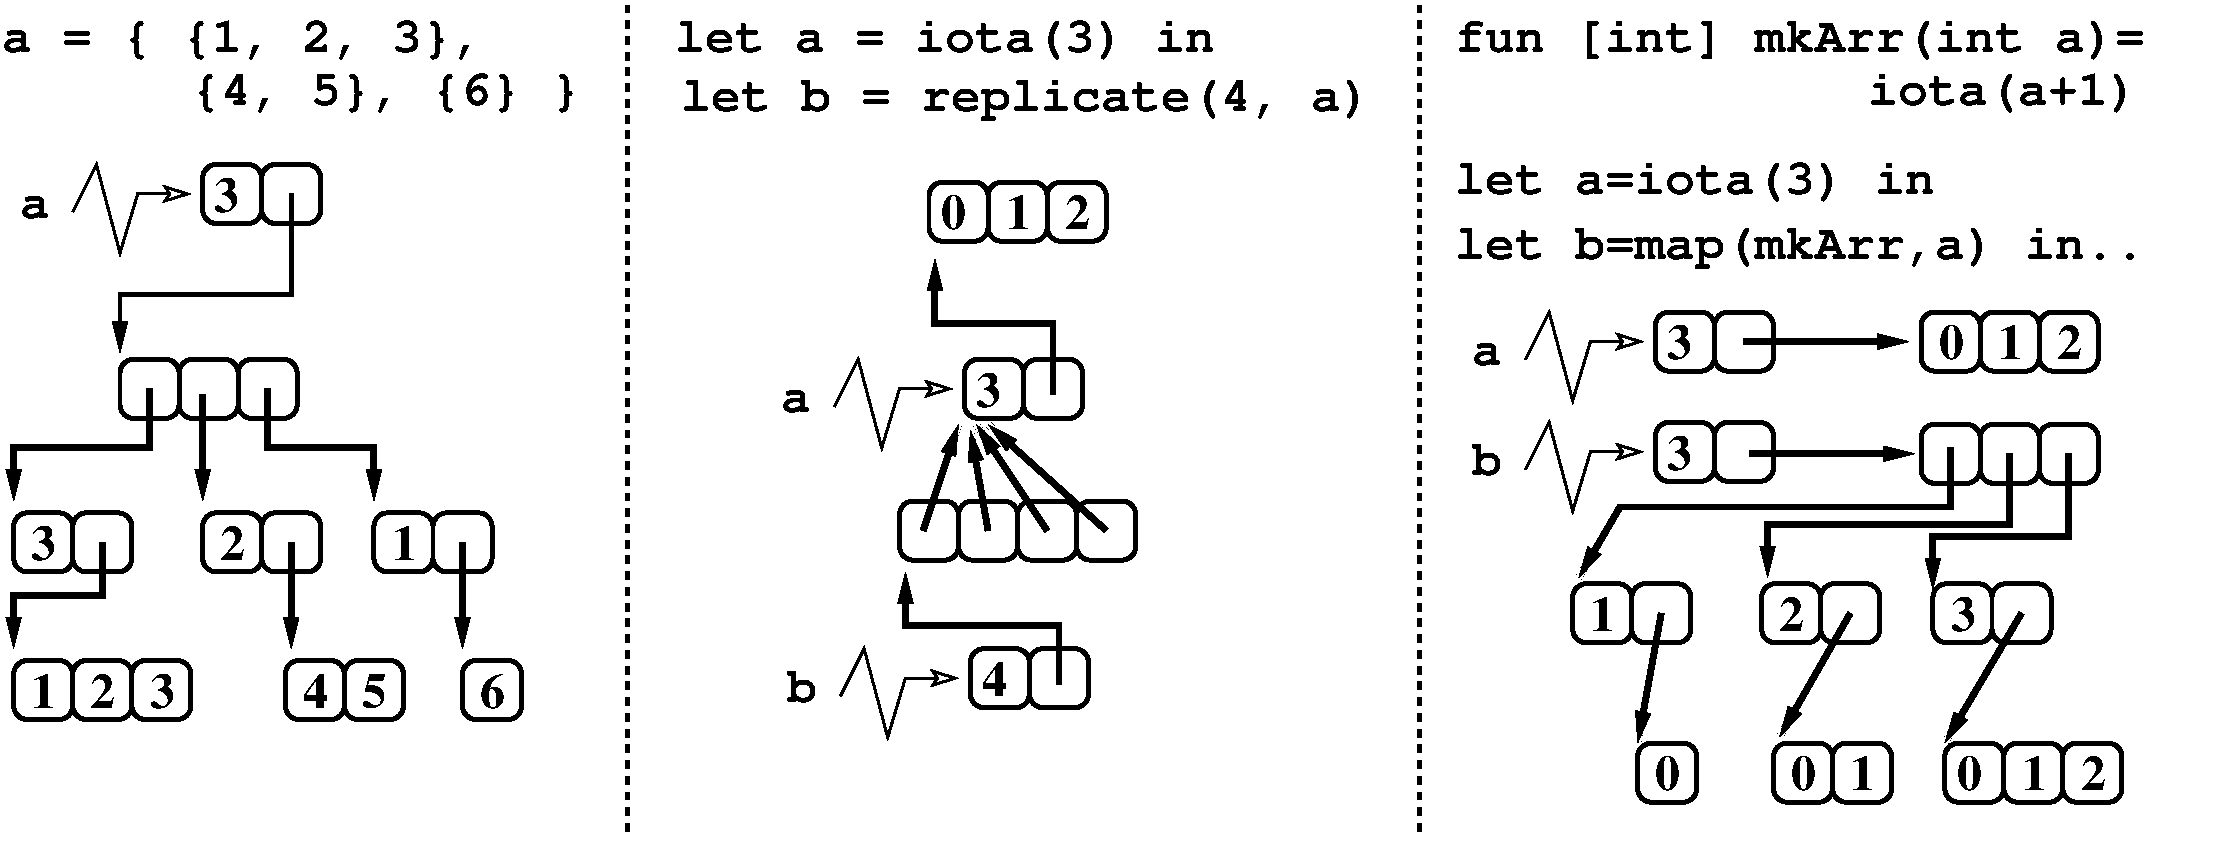
\includegraphics[scale=0.33]{Figures/Arrays}
%\includefigure[scale=1.5]{Figures/Arrays}
\hrule
\vspace*{-1ex}
\caption{Array Layout.}
\label{fig:ArrLayout1} %
\vspace*{-1ex}
\end{figure}

Figure~\ref{fig:ArrLayout1} illustrates the array representation used in
the \mips{}32 code generator on several code examples. 
%
In essence, a \fasto array, named {\tt arr}, is 
implemented by a two-word header, where the first word holds the 
{\it length} of the (outer dimension of the) array, named $N$, and the second 
word holds the address of the array's {\it content}. 
%
The content is a contiguous \emph{word-aligned} chunk of memory big enough 
to store all array elements. If {\tt arr :{}[bool]} then its size is 
$(N+3)/4$ words, which holds at least $N$ bytes. Arrays of type {\tt [char]}
have an extra {\tt '0'} element at the end (for printing), making the content size 
$(N+4)/4$ words (which holds at least $N+1$ bytes).
If {\tt arr :[int]}, the content size is $N$ words, as the size of integer is one word.
The same applies if an array is multidimensional: its content holds pointers (one word each)
to arrays of lower dimensions. Note that several elements of an array may point
to the same (lower-dimensional) array, as shown in Fig.~\ref{fig:ArrLayout1}.


\section{Project Tasks}
\label{sec:Tasks}

\subsection{\fasto Features to Implement}


Your task is to extend the implementation of the \fasto compiler in
several ways, which are detailed below. To ``extend the implementation'' means
to do whatever is necessary for (i) legal programs to be {\em interpreted} and
{\em translated} to \mips code correctly, and for (ii) all illegal programs
to be rejected by the compiler. 

\newcounter{taskCnt}
\setcounter{taskCnt}{0}
\newcommand{\nexttask}{\addtocounter{taskCnt}{1}\arabic{taskCnt}}

\paragraph{\nexttask. Warm-Up: Multiplication, division, boolean operators 
and literals.}

Add the operators and boolean literals given below to the expression 
language of \fasto, and implement support for them in all
compiler parts: lexer, parser, interpreter, type checker, \mips code
generator. 
This task aims to get you acquainted  with the compiler
internals.
The implementation of these operators will be very similar to other,
already provided, operators.

\vbox{ 
$
\begin{array}{lclr}
Exp & \rightarrow & Exp \mbox{ }{\tt{}*}\mbox{ } Exp & {\tt (* integer-multiplication \mbox{ }operator *)}\\
Exp & \rightarrow & Exp \mbox{ }{\tt{}/}\mbox{ } Exp & {\tt (* integer-division \mbox{ }operator *)}\\ [0.9ex]

Exp & \rightarrow & Exp \mbox{ }{\tt{}\&}\mbox{ } Exp & {\tt (* boolean-and \mbox{ }operator *)}\\
Exp & \rightarrow & Exp \mbox{ }{\tt{}|}\mbox{ }\mbox{ } Exp & {\tt (* boolean-or  \mbox{ }operator *)}\\ [0.9ex]

Exp & \rightarrow & {\tt{}True} & {\tt (* boolean-true \mbox{ }value *)}\\
Exp & \rightarrow & {\tt{}False} & {\tt (* boolean-false  \mbox{ }value *)}\\ [0.9ex]

Exp & \rightarrow & \mbox{ }{\tt{}not}\mbox{ } Exp & {\tt (* boolean-negation \mbox{ }unary\mbox{ }operator *)}\\
Exp & \rightarrow & \mbox{ }{\tt{}\sim}\mbox{ }\mbox{ } Exp & {\tt (* integer-negation \mbox{ }unary\mbox{ }operator *)}\\ [0.9ex]
\end{array}
$
}

As usual, multiplication and division bind stronger than addition and subtraction.
Likewise, the \texttt{\&} operator binds stronger than the \texttt{|} operator, and both 
should be left-associative. Logical negation binds stronger than \texttt{\&} and \texttt{|}.
Logical operators should not bind stronger than comparisons. Examples:

\begin{itemize}
\setlength{\itemsep}{0ex}
\setlength{\parskip}{0ex}
\item \texttt{\small to = be | not to \& be = True} means 
\texttt{\small (to=be) | ((not to)\&(be=True))}
\item \texttt{ $\sim$ a + b * c = b * c - a} means \texttt{ (($\sim$a)+(b*c)) = ((b*c)-a)}
\end{itemize}

\paragraph{\nexttask. Bounds Checking for the Array Index Operation.} 

%The next task is to implement bounds checking in
%the {\tt Mips} code-generation phase. 
Currently, the behaviour of the implementation is undefined when 
indexing an array outside its bounds, e.g., {\tt a[$\sim$1]}.
Extend the code generation for array indexing in {\tt compileExp}
to check the index value and terminate the program
execution with an error message if the value is not within $0$ and 
the array size minus one.   Place your implementation in function
{\tt check\_bounds}, which is currently empty.
%
The implementation already checks that the size argument of \texttt{iota} and
\texttt{replicate} is greater than zero.  Implement the index-out-of-bounds error
in the same way. In particular, the error message should contain the position of 
the failing index operation in the source code.

%Implement the {\tt check\_bounds} function, currently empty, which 
%is called from the implementation of {\tt compileExp} corresponding to the 
%{\tt Fasto.Index} type constructor.   Your implementation of {\tt check\_bounds}
%is required to verify whether the index is within legal bounds of the corresponding
%array, and if not, execution will jump to handler {\tt \_IndexError\_}, which will 
%report the program's line number at which the index-out-of-bounds exception has
%occurred. 
%(You are responsible to passing the proper line number to {\tt \_IndexError\_}.
%Note also that it is possible to implement {\tt check\_bounds} in $10$ lines of code).

\paragraph{\nexttask. Built-In Operators/Functions Used Directly in \textsc{soac}:} 
%
This task is to allow unary operators ({\tt $\sim$} and \texttt{not}) to be passed
directly as the function parameter of {\tt map}. For this the \fasto's grammar
needs to be extended such that the first argument of {\tt map} can be the 
keyword {\tt op} followed by an operator symbol.
%
Similar changes should be made for the {\tt reduce} function (allowing {\tt op} followed by
a binary operator, i.e., {\tt +, *, \&, |}, as the first parameter). % {\tt zipWith}, and {\tt scan}.  
For instance the following code should become legal in \fasto: 

\vspace{-1ex}
\vbox{ \begin{Verbatim}
fun int main() =                 fun [int] main() = 
  let x = iota(10) in                let x = iota(10) in
  reduce(op +, 0, x)                 map(op ~, x)  
// 0+0+1+..+9=45                 // {0, -1, -2, .., -9}  
\end{Verbatim}
}\vspace{-1ex}


The implementation strategy is your choice. For example a valid approach
would be to design a source-to-source translation that constructs a new 
abstract-syntax representation (\textsc{AbSyn})
in which (i) a uniquely named function is created for each such operator, i.e.,
{\tt fun int plus(int a, int b) = a + b}, and in which (ii) calls
such as {\tt reduce(op +,..)} are replaced with {\tt reduce(plus,..)}. 


\paragraph{\nexttask. Implement \emph{either} (i) \texttt{zipWith} and
\texttt{write} \emph{or} (ii) \texttt{scan} and \texttt{length}.}
The handed-out \fasto implementation only supports \texttt{map} and
\texttt{reduce} as second-order array combinators.  One part of the task is to
add support for \texttt{zipWith} or \texttt{scan}, as described in
Sections~\ref{subsec:map-red-prog}~and~\ref{subsec:hof-implem}.  The operations
need to be added to all compiler phases.
Make sure you understand how \texttt{map}
and \texttt{reduce} are handled, then the implementation of \texttt{zipWith}
and \texttt{scan} should be straightforward.  Type-checking for
\texttt{zipWith} is (a bit) more difficult then for \texttt{scan}, and they
both require roughly the same implementation effort in the code generation
phase. 

The second part of the task is to implement one of the (polymorphic) built-in
functions \texttt{length} and \texttt{write}, which will now operate on arrays
of arbitrary types.
%
Function \texttt{length : [a] $\rightarrow$ int} returns the length of an
arbitrary array, i.e., the number of elements in the array's outer dimension.
The machine code for \texttt{length} should be ``short and straightforward'',
while type checking requires slightly more work.
%
Function \texttt{write} currently works only on basic types and on arrays of
characters (and string literals), but you will extend the implementation to
print arbitrary arrays.  The type-checker needs to be relaxed to allow this
more general use of \texttt{write} (easy), and the interpreter and code
generator need to be extended to traverse and print the array elements.
Printing multidimensional arrays will require recursive calls to code
generation.
%
With both extensions, the code below should be legal: \texttt{fun int main() = write(
map(length, \{ "abc", "de", "f" \} ) )} \\ and the output could possibly be:
\texttt{\{ 3 2 1 \}}.

{\em Implement either (i) {\tt zipWith} and {\tt write} or (ii)
{\tt scan} and {\tt length}}.

\paragraph{\nexttask. Dead-Function Elimination.}

Dead-Code Elimination is an optimization to remove code which does not affect
the program results. This shrinks the program size and avoids the execution of
irrelevant operations.

Implement a source-to-source translation of the abstract syntax tree which
removes all unused functions from the program, i.e., functions that are defined
but are never called during execution. Do this by extending the function {\tt
live\_funs} in the file {\tt Optimization.sml}. The function {\tt live\_funs}
has the signature

%The last task is to implement a source-to-source translation
%at the \textsc{AbSyn} level, which removes all unused functions from the program,
%i.e. functions which are defined but will never be called during execution.
%
%The core of the implementation is a function {\tt live\_funs} with the following signature, argument description and return value:
%\vspace*{-2ex}
\begin{fancycode}[fontsize=\small]
Fasto.Exp * string list * (string * Fasto.FunDec) list -> string list
\end{fancycode}
%\vspace*{-2ex}

The arguments are
(i) a \fasto expression, {\tt exp},
(ii) a list of already known to be reachable function names, {\tt alive}, and
(iii) a function symbol table, {\tt ftable}.

The return value is a list of {\em all} function names that are called during
the execution of {\tt exp}, including the ones already {\tt alive} before. It
is not necessary to consider whether program logic prevents a function call
from being made. The result list must not contain duplicate names.

The idea is to build the result recursively by accumulating the contributions
of all child expressions of {\tt exp}.  If {\tt exp} involves a function name,
{\tt fname}, e.g. by being {\tt Apply}, {\tt Map} or {\tt Reduce}, this
function also needs to be investigated. If {\tt fname} is not already in {\tt
alive}, the function is added and its body is searched for other functions that
could be called from {\tt fname}.


\subsection {Testing your Solution, Input (\fasto) Programs}
\label{InpPrgs}

It is your responsibility to test your implementation thoroughly.
Please provide the test files in your group submission.
%
As a starting point, some input programs can be found 
in folder {\tt DATA}. Among them:

\begin{itemize}
\setlength{\itemsep}{0.1ex}
\setlength{\parskip}{0.1ex}
    \item {\tt fib.fo} computes the {\tt n}$^{th}$ Fibonacci number.
    \item {\tt testBuiltIn.fo} tests the built-in functions.
    \item {\tt ArrayLitWrite.fo} tests the write operation on bi-dimensional arrays of
            basic types {\tt bool}, {\tt char}, and {\tt int}.
    \item {\tt SimpleIota.fo} and {\tt SimpleReduce.fo} test programs with {\tt iota} and {\tt reduce}.
    \item {\tt SimpleRead.fo} and \texttt{testRead.fo} test the read function.
    \item {\tt InlineMap.fo} and {\tt OptSimple.fo} test the optimizations. 
    \item {\tt testIOMSSP.fo} implements the non-trivial algorithm for solving the
            ``maximal segment sum'' problem.
    \item {\tt error-01-type.fo} tests a simple type error (compilation will fail),
    	and {\tt runtime-error-00-iota-zero.fo} compiles, but fails at runtime.
\end{itemize}

If a test program \texttt{\textit{foo}.fo} has a corresponding
\texttt{\textit{foo}.in} file, the program is intended to compile
correctly, and produce the output in \texttt{\textit{foo}.out} when
run with the input from the input file.  If no input file exist, the
program is is invalid, and the compiler is expected to report the
error in \texttt{\textit{foo}.err}.

You should extend and modify these test cases to test the new features
you have added.  You can add new test programs by following the naming
convention outlined above.
%
Tests can be run on a Unix-compatible platform using the
\texttt{testg.sh} script in the \texttt{SRC} directory.  Standing in
the \texttt{SRC} directory, run

%\vspace*{-1ex}
\begin{verbatim}
      $ ./testg.sh
\end{verbatim}
%\vspace*{-1ex}

This will recompile the compiler, then compile and run every test
program found in the \texttt{DATA} directory, comparing actual output
with expected output.  If \texttt{testg.sh} complains that it cannot
find \mars, run the script as follows:

%\vspace*{-1ex}
\begin{verbatim}
      $ MARS=/path/to/Mars_4_2.jar ./testg.sh
\end{verbatim}
\noindent
where \texttt{/path/to/Mars\_4\_2.jar} is the path to \mars.

On Windows, you may have luck running \texttt{testg.sh} with
MSYS\footnote{\url{http://mingw.org/wiki/msys}} or
Cygwin\footnote{\url{http://cygwin.com/}}.  Of these, Cygwin is more
heavyweight, but also more likely to work.

\subsection{Partitioning Your Work}

The solution and report have to be completed within five weeks time.
While you may be tempted to
postpone work on the task towards the end of the period, this would be a bad 
idea. Instead, try to work on the parts described in the lecture, 
making the required changes in respective compiler modules and describing
this part of your work in the report. 
It is a good idea to reserve the last week to report writing and testing.

In particular, \emph{tasks $1$ and $4$} require changes to all compiler phases.
Try to implement each part of them immediately after the corresponding
lecture. It is even possible to \emph{start task $1$ immediately} after you
learn about parsing, because the rest of the code can be ``pattern matched''
from similar, already implemented, code.  

\emph{Task $2$} can be completed immediately after the intermediate/machine-code
generation lecture. It should not take more than two hours.
\emph{Tasks $3$ and $5$} can be completed immediately after building the 
abstract-syntax tree (\textsc{AbSyn}) of the input program, i.e., after
parsing, as they require (only) an \textsc{AbSyn}-level translation.
   
\nocite{PattersonHennessy}
\nocite{Torben2011}
%\nocite{TorbenDIKU}
\nocite{MipsModule}

\bibliographystyle{unsrt}
\bibliography{CB12}
%\bibliography{GroupProj}

%%%%%%%%%%%%%%%%%%%%%%%%%%%%%%%%%%%%%%%%%%%%%%%%%%%%%%%%%%%%%%%%%%
%%%%%%%%%%%%%%%%%%%%%%%%%%%%%%%%%%%%%%%%%%%%%%%%%%%%%%%%%%%%%%%%%%
%%%%%%%%%%%%%%%%%%%%%%%%%%%%%%%%%%%%%%%%%%%%%%%%%%%%%%%%%%%%%%%%%%
\newpage
\appendix

\part*{Appendix}
\addcontentsline{toc}{part}{Appendix: Description of the \fasto Compiler Modules}
\section*{Description of the \fasto Compiler Modules}
\label{sec:modules}

We provide an implementation of the \fasto compiler as a basis for the tasks
described above. This section introduces the compiler's structure and 
explains some details and reasons for particular choices.

\subsection*{Lexer, Parser and Symbol Table}

The lexer and parser are implemented in files 
{\tt Lexer.lex} and {\tt Parser.grm}, respectively. 
The lexical rules have been already described in Section~\ref{subsec:lexicalrules},
and the grammar has been shown in Figure~\ref{fig:FastoGram1}.

File {\tt SymTab.sml} provides a polymorphic implementation of the 
symbol table.   The symbol table is simply a list of tuples, in which
the first term is a string, denoting the name of a variable/function, and the
second term is the information associated to that name. The type of 
the second term is polymorphic, i.e., different types of information will be stored
in different tables during processing.
The main functions are: (i) {\tt bind}, which adds a name-value pair to 
the symbol table (potentially hiding an older entry), and (ii) {\tt lookup}. 
Function {\tt lookup} receives
as input the name of a variable, {\tt n}, and searches the symbol table to find 
the closest binding for {\tt n}. If no such binding exists then option {\tt NONE}
is returned, otherwise {\tt SOME m}, where {\tt m} is the information
associated with {\tt n}. 
A variant \texttt{insert} of \texttt{bind} raises an exception when an old entry
would be hidden by a new one.

\subsection*{Abstract Syntax Representation}
\label{subsec:AbSyn}

The abstract-syntax representation is defined in file 
{\tt Fasto.sml}: the entire program has type {\tt Fasto.Prog}, which is a
list of function declarations. A function declaration has type {\tt Fasto.FunDec}. 
Expressions and types are build by the constructors of types 
{\tt Fasto.Exp} and {\tt Fasto.Type}, respectively, and so on. 

Note that several type constructors of {\tt Fasto.Exp} contain
{\tt Fasto.Type} nodes, which are initialized to 
{\tt Fasto.UNKNOWN}, for instance the indexing constructor is declared as {\tt Index of string * Exp * Type * pos}.  
These type nodes are replaced by the correct type by the type checker, 
and used in the \mips code generation phase. For example,
generating \mips code for array indexing ({\tt a[i]}) 
requires to know whether the element type is stored in one byte or
in one word (four bytes), i.e., whether to use a load-byte or load-word instruction.

{\tt Fasto.sml} also provides functions 
to pretty print a program ({\tt prettyPrint}),
a function ({\tt pp\_fun}), a type ({\tt pp\_type}), or
an expression ({\tt pp\_exp}).   Pretty printing can be used 
for user-friendlier error messages and for debugging. 
%
Also, when a correct abstract syntax tree is \texttt{prettyPrint}ed, 
the resulting string should again be valid input to the compiler and lead 
to the same abstract syntax tree.

\subsection*{Interpreter}

The Interpreter is implemented in file {\tt Interpret.sml},
and its signature is given in file {\tt Interpret.sig}. 
The entry point is function {\tt evalPgm}, which builds the
symbol table for functions and starts the interpretation of the 
program by interpreting function {\tt main}.
%
Interpreting a (call to a) function is implemented by function
{\tt callFun}, which: (i) evaluates the function arguments, 
(ii) creates a new symbol table for variables and binds the evaluated
arguments to the function's formal arguments, and (iii) continues
by interpreting the expression that corresponds to the body of the function.
%
Finally, interpreting an expression is implemented by {\tt evalExp}
via case analysis on the type constructors of {\tt Fasto.Exp}.

\subsection*{Type Checking}

The type checker is implemented in file {\tt Type.sml},
and its signature is given in file {\tt Type.sig}. 
The entry point is {\tt checkProgram : Fasto.Prog $\rightarrow$ Fasto.Prog},
which verifies that all functions in the program have the declared type.

Type checking a function means to verify that the result type of the function
matches the type of the function-body expression, given the formal parameters
have the declared types.
Typechecking a function \emph{application} means to verify that the types of 
the actual and the formal parameters match.
%
Expressions are type-checked recursively, building types in a bottom-up fashion.
For instance, type-checking an {\tt if-then-else} means to
check that the condition is boolean, and to determine the types of the {\tt then}
and {\tt else} sub-expressions and to verify that these types are the same.
%
Type checking an expression is mainly implemented by {\tt expType}
via case analysis on the type constructors of {\tt Fasto.Exp}.
{\it Your changes to the type checker will mainly 
extend {\tt expType}'s implementation.}

As mentioned, type information also needs to be passed to the \mips code 
generator, especially for arrays and for the built-in \texttt{write} function.
Therefore, {\tt checkProgram} builds a new abstract-syntax
representation in which the type information of various
{\tt Fasto.Exp} constructors are changed from {\tt UNKNWON} to the correct types
(for instance the type of the array for array-indexing \texttt{a[i]}).

\subsection*{High-Level Optimizations}

Several code transformation at the abstract-syntax-representation level 
are implemented in file {\tt Optimization.sml}.
The entry point in the optimization module is function {\tt opt\_pgm}, which
first renames all variable names in all functions to (new) unique names 
(via the use of {\tt unique\_rename}), and then calls function {\tt opt\_fixpoint},
which applies a set of code transformations to a fix point, i.e., until no further
changes are possible.
%
\begin{itemize}
    \item {\em Let Normalization} attempts to bring {\tt let} expressions 
            to a normal form, e.g., \\
            {\tt let x = (let a = iota(n) in map(f,a)) in reduce(plus,0,x)} \\
            will be transformed via function {\tt let\_norm\_exp} to \\
            {\tt let~a=iota(n)~in~let~x=map(f,a)~in~let~t=reduce(plus,0,x)~in~t}.
    \item {\em Inlining} performs aggressive function inlining: at every stage,
            if a function does not call any other function directly
            (calls via {\sc soac} {\tt map} and {\tt reduce}
            are not considered), its body is inlined at every call site.
            The inlining process is then repeated until no further inlining is 
            possible (fix point), because inlining a
            function may create new opportunities for inlining other functions. 
            The implementation's entry point is function {\tt inline\_driver}. 
    \item {\em Map Fusion} replaces nested calls to \texttt{map} by function composition,
    	    using the invariant
            {\tt map(g, map(f, a)) $\equiv$ map(g o f, a)}. The expression on the right-hand
            side does not materialize the intermediate array {\tt map(f,a)} in memory, 
            thus memory consumption is reduced considerably.
%
            The implementation is careful to only remove arrays which
            are not used elsewhere, e.g., with the code
            {\tt let b = map(f, a) in let c = map(g, b) in \emph{exp}}, the two
            {\tt map}s are fused to {\tt let c = map(g o f, a)} only if
            {\tt b} is not used inside \emph{exp} any more. 
            One could replace several occurrences of {\tt b} by \texttt{map(f,a)},
            but if {\tt f} is expensive to compute, the program
            might run slower because {\tt map(f,a} is computed several times.
            The implementation's entry point
            is {\tt mapfusion\_driver}. 
\end{itemize}

Note that you are not required to understand the details pertaining to the
implementation of these transformations.   We provide them just to demonstrate
examples of high-level optimizations.

\subsection*{Register Allocator}

The register allocator is implemented in {\tt RegAlloc.sml}
and its associated signature can be found in {\tt RegAlloc.sig}.
{\it The project will not require changes to the register-allocator 
implementation.}

\subsection*{\mips Code Generation}

Code Generation for the \mips architecture is implemented in file 
{\tt Compiler.sml} and its signature is given in file {\tt Compiler.sig}. 
The entry point is {\tt compile : Fasto.Prog $\rightarrow$ Mips.mips list},
which takes as input the abstract-syntax representation of the input
program and generates a list of \mips instructions.
%
The type constructors for \mips instructions are implemented
in file {\tt Mips.sml}, i.e., {\tt datatype Mips}, together with 
the functionality to print them, i.e., {\tt pp\_mips} and
{\tt pp\_mips\_list}. 

Function {\tt compile} generates \mips code for all functions declared in the program
(via \texttt{compileFun}), and combines the resulting code
with static code that initializes constants and executes the \texttt{main} function,
also adding standard {\sc io} routines ({\tt put/getint} and {\tt put/getstring})
and code for exception handling ({\tt \_IllegalArrSizeError\_}).
%
Documentation on the \mips instruction set and the mechanism 
via which functions are called is provided in file {\tt mips-module.pdf}.

Code generation for an arbitrary \fasto expression is 
achieved via function
\vspace*{-2ex}
\begin{fancycode}
compileExp: Fasto.Exp*(string*string)list*string -> Mips.mips list
\end{fancycode}
\vspace*{-2ex}
Its first argument is the expression to generate code for,
the second argument is the symbol table for variables, 
which associates a variable name with the name of the symbolic
register that holds the variable's value, and the third 
argument is the name of the symbolic register where the result
of the expression is to be placed. The implementation of
{\tt compileExp} is done by case analysis on the type constructors
of {\tt Fasto.Exp}.   
{\it The \fasto 
extensions to implement in the tasks will mainly require
extensions to {\tt compileExp}}.
   

\subsection*{\mips Code Generation: Array Layout}

We implement an array of integers of length {\tt n} via the following
representation: We allocate a header of 2 (four-byte) words, and a content 
area of {\tt n} words. The header holds holds the length of the array, 
{\tt n}, and a pointer to the content area (the content will often follow
right behind the header, but this is not required in the design).
The content area of {\tt n} words holds the values of the array. 
The array heap is implemented as reserved data space in the compiled program
pointed at by a heap pointer. Allocation of memory simply means to increment
the heap pointer by the corresponding amount, the previous value points to 
the allocated memory.

\begin{figure}[t]%[tbh]
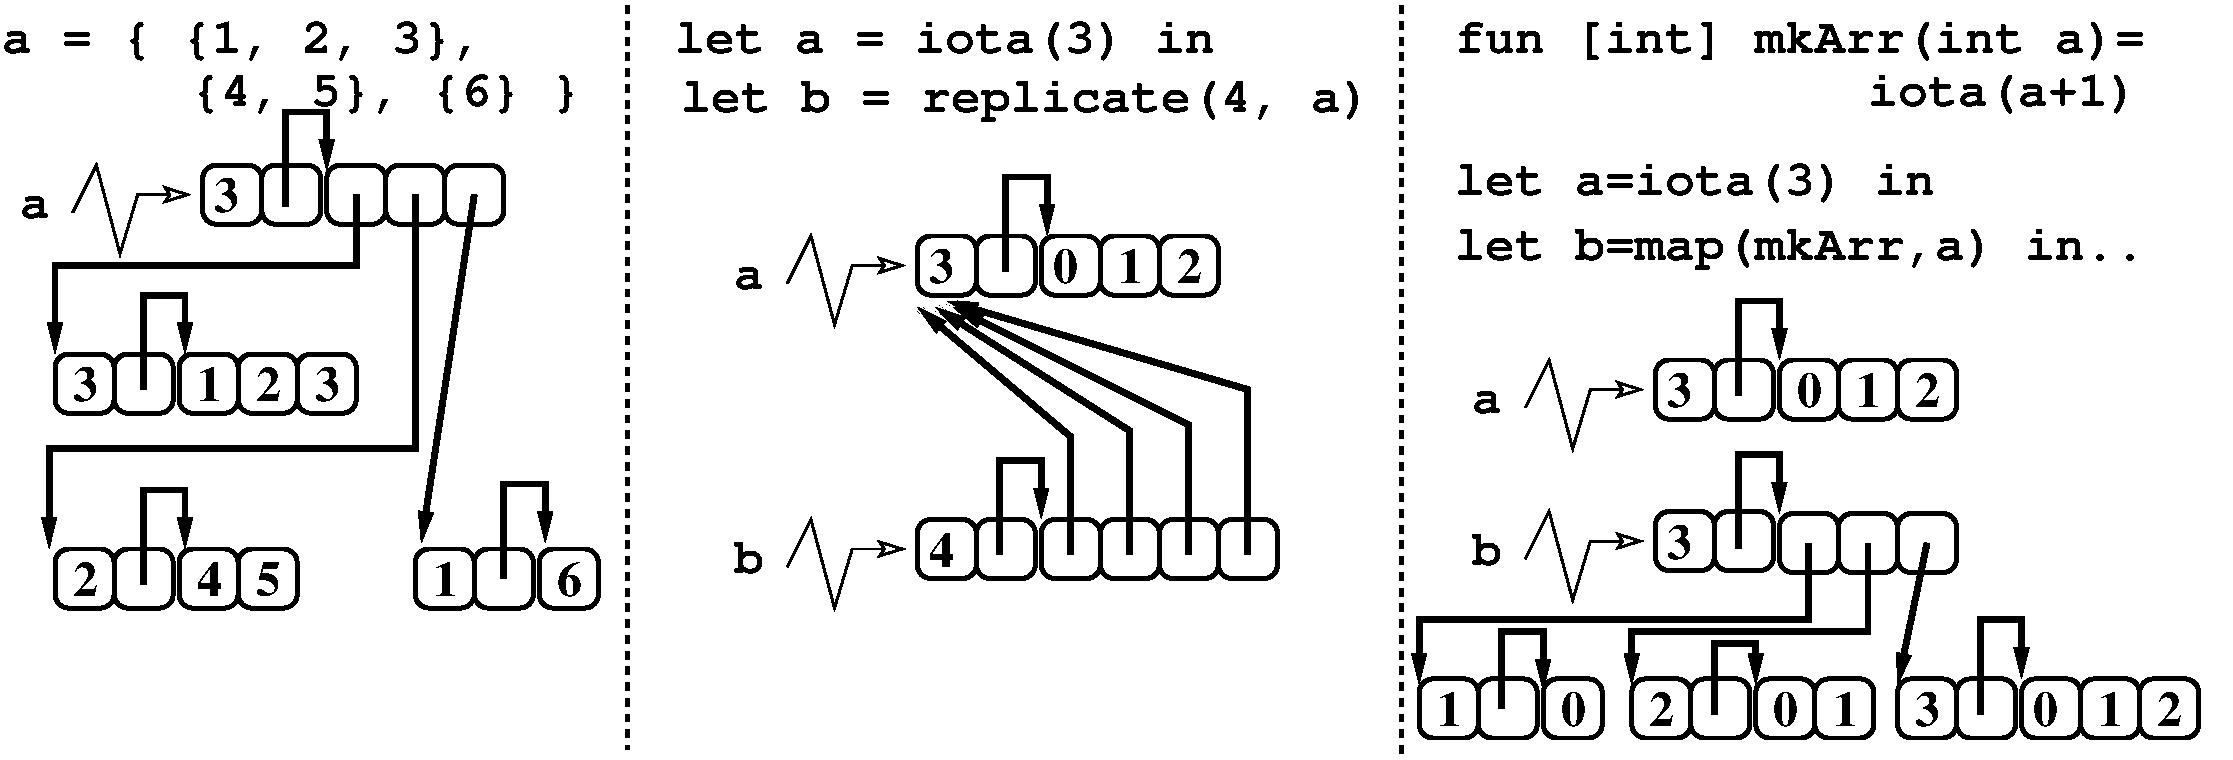
\includegraphics[scale=0.35]{Figures/ArraysPrecise}
%\includefigure[scale=1.5]{Figures/Arrays}
\hrule
\caption{Array Layout.}
\label{fig:ArrLayout} %
\end{figure}

An array of booleans or characters is implemented similarly, the only difference
is that each array element requires only one {\tt byte}
rather than one word (4 bytes). On the other hand, memory allocation in the heap 
need to be \emph{word-aligned}, to avoid runtime failures caused by load-word instructions.
It follows that for an array of booleans we allocate
{\tt (n+3)/4} words of content space (rounding up to a full word).
Again, two words are allocated for the array header (length and content pointer),
and the content space is at least {\tt n} bytes holding the array's elements.
An array of characters is handled similarly, but an extra \texttt{0} character
is added at the end, making its length logically {\tt n+1} bytes.
Therefore, {\tt (n+4)/4} words are allocated for the content, and we write {\tt 0} as 
the last character. This is done in order to allow for printing the array as a string 
using the {\tt putstring} system call.
%
Finally, a multi-dimensional array requires the same allocation as an array of integers,
however the array elements are now (word-sized) pointers to other arrays.
%(We have assumed that the size of an integer 
%equals the word size, i.e., four bytes with \mips.)

Figure~\ref{fig:ArrLayout} depicts and demonstrates the array layout 
on three code examples.  The leftmost example shows a bi-dimensional
array of literals: the representation of {\tt a} is a pointer to
an array header holding value \texttt{3} and a pointer to the 
(immediately following) content space of 3 words. The three array elements are pointers
to the inner arrays: The first inner array has length {\tt 3} 
and elements {\tt 1,2,3}, the second has length {\tt 2} and
elements {\tt 4, 5}, and the third one has length {\tt 1} 
and content {\tt 6}. Note that the inner arrays have a similar
representation.

The example in the middle of Figure~\ref{fig:ArrLayout} replicates 
array {\tt a = iota(3) = \{0, 1, 2\}}
four times. The result array {\tt b} is thus an array of size {\tt 4},
i.e., the first word in its representation holds value {\tt 4},
and the content of the array consists of four identical pointers pointing to
array {\tt a}. 
%
Finally the rightmost example uses {\tt map} to create a bi-dimensional array, {\tt b},
of three rows, in which the first, second and third rows have one, two and three
elements, respectively.   The array structure is similar to the one of the
array {\tt a} in the leftmost example.

\subsection*{\mips Code Generation Case Study: Iota and Map}

This section describes the \mips translation for 
the array-producing functions {\tt iota} and {\tt map}.
We start with  the high-level intuition, and then
we present the structure of the code that implements the
corresponding \mips translation. 

\vbox{ \begin{Verbatim}
let x = iota(n) in ...              x = dynalloc((n+2)*4); 
                                    x[0] = n; x[1] = &(x[2]);
                                    for(i=0, i<x[0]; i++)
                                        x[i+2] = i;
\end{Verbatim}
}

\noindent The code snippet above suggests a translation of 
{\tt x = iota(n)} to the {\tt C}-like code on the right-hand side: 
{\tt dynalloc} allocates space for {\tt n+2} words, then the
first word is set to {\tt n}, the resulting-array size, and the
second word points to the content of the array, i.e., the third word.
The {\tt for} loop fills the content of the array with the first
{\tt n} natural numbers (starting from $0$), corresponding to {\tt iota}'s
semantics. 


\vbox{ \begin{Verbatim}
fun int plus2(b) = b + 2            x = dynalloc((a[0]+2)*4); 
fun int main() =                    x[0] = a[0]; x[1] = &(x[2]);
  let x = map(plus2, a)             for(i=0, i<x[0]; i++) {
  in ..                                 x[i+2] = plus2(a[i+2]);
\end{Verbatim}
}

{\tt map} is treated similarly, the only differences being that
(i) the size of the result array, {\tt x}, is found by inspecting the size 
of the input array, {\tt a}, and (ii) the elements of {\tt x} are computed
by applying/calling function {\tt plus2} on the corresponding elements of 
{\tt a}.  Obviously, parts of the code are the same as for \texttt{iota},
and the implementation will use helper functions to generate those parts.

\vbox{ \begin{Verbatim}
fun compileExp e vtable place =
  case e of
  ........
  | Fasto.Iota (n, pos) =>
      let val sz_reg  = "_size_reg_"^newName()
          val code_sz = compileExp n vtable sz_reg
          fun funel(i,r) = [Mips.MOVE(r,i)]
      in  code_sz @ dynalloc( sz_reg, place, Fasto.Int(pos) ) @ 
          compileDoLoop( 4, sz_reg, place, funel, pos )
      end
\end{Verbatim}
}
\noindent The code above implements the \mips code generation for {\tt iota}:
First, a new symbolic register is created, {\tt sz\_reg}, 
and the recursive call to {\tt compileExp} generates the code
that will compute {\tt iota}'s argument, {\tt n}, where the
result of evaluating {\tt n} will be ``placed'' in {\tt sz\_reg}. 


Second, we define function {\tt funel} that generates the code that will compute
the value to be stored in the {\tt i}$^{th}$  element of the result 
array ({\tt (i+2)}$^{th}$ with our array layout).  The arguments of {\tt funel}
are the symbolic register that stores the loop counter {\tt i} and 
the result register {\tt r}. The implementation simply moves the value
of the loop counter to the result register, since for {\tt iota},
the {\tt i}$^{th}$ element is exactly the loop counter {\tt i},
i.e., {\tt a[i] = i;}.

Third, (i) the code that computes {\tt n}, i.e., {\tt code\_sz}, is
merged with (ii) the code generated by helper function {\tt dynalloc},
which allocates memory for the result array and fills in the array's header, 
i.e., the first two words, and with (iii) the code that implements the
loop. The latter code is computed via helper (and second-order) function 
{\tt compileDoLoop} that receives as argument (and uses) function {\tt funel} 
in order to generate the loop structure  {\tt for(i=0, i<x[0]; i++) x[i] = i;}.

 Finally, the code that implements \mips-code generation for {\tt map}, 
given below, exhibits a similar structure:  First, {\tt compileExp} is 
recursively called to generate the code that stores the input-array address in
symbolic register {\tt arr\_reg}.

\vbox{ \begin{Verbatim}
fun compileExp e vtable place =
  case e of
  ........
  | Fasto.Map  (fid, arr, eltp, rtp, pos) => 
      let val arr_reg = "_arr_reg_"  ^newName()
          val inp_addr= "_arr_i_reg_"^newName() 
          val sz_reg  = "_size_reg_" ^newName()
          val arr_code  = compileExp arr vtable arr_reg

          fun funel(i, r)=if ( getElSize eltp = 1 )
                          then Mips.LB(r, inp_addr, "0")
                            :: ApplyRegs(fid, [r], r, pos) 
                            @ [Mips.ADDI(inp_addr,inp_addr,"1")]
                          else Mips.LW(r, inp_addr, "0")
                            :: ApplyRegs(fid, [r], r, pos)
                            @ [Mips.ADDI(inp_addr,inp_addr,"4")]
      (*** we use sz_reg to hold the input/output-array size***)
      in arr_code @ [ Mips.LW(sz_reg, arr_reg, "0")] @ 
         dynalloc(sz_reg, place, rtp) @ 
         [Mips.LW(inp_addr, arr_reg, "4")] @
         compileDoLoop(getElSize rtp, sz_reg, place, funel, pos)
      end
\end{Verbatim}
}

\enlargethispage{\baselineskip}

Second, function {\tt funel} is defined: (i) {\tt inp\_arr} implements an
iterator of the input array, (ii) the current element is stored in symbolic
register {\tt r}, (iii) the helper function {\tt ApplyRegs} generates the code
that calls/applies {\tt map}'s input function {\tt fid} on {\tt r} and stores 
the result back into {\tt r}, and (iv) finally, {\tt inp\_addr} iterator is
incremented to point to the next array element.   Note that the size of
the array's element type, {\tt el\_tp}, is used to discriminate between the boolean/character
and integer cases. With the former, the load byte ({\tt LB}) instruction is used
(instead of load word, {\tt LW}), and {\tt inp\_addr} is incremented with one
byte (rather than four bytes).  

Finally, (i) the code that computes the input-array address, {\tt arr\_code}, 
is merged with (ii) the code that loads the input-array size in register {\tt sz\_reg}, i.e., \\
{\tt [ Mips.LW(sz\_reg, arr\_reg, "0")]}, with (iii) the result of {\tt dynalloc},
with (iv) code to initialize the input-array iterator, i.e., \\
{\tt [Mips.LW(inp\_addr, arr\_reg, "4")]}, and with the code that generates the loop,
i.e., {\tt compileDoLoop(getElSize rtp, sz\_reg, place, funel, pos)}.


\subsection*{\fasto Compiler Driver}

The main driver of the (whole) compiler resides in file
\texttt{SRC/FastoC.sml}, and the executable will be generated in
\texttt{BIN/FastoC}. To interpret an input program located in file
\texttt{DATA/filename.foo}, run

\vbox{ \begin{verbatim}
$ BIN/FastoC -i DATA/filename
\end{verbatim}
}

To compile-to/generate \mips code while applying the high-level optimizations,
run

\vbox{ \begin{verbatim}
$ BIN/FastoC -o DATA/filename
\end{verbatim}
}

To compile-to/generate \mips code without applying the high-level
optimizations, run

\vbox{ \begin{verbatim}
$ BIN/FastoC DATA/filename
\end{verbatim}
}

This will generate file \texttt{DATA/filename.asm} that you can run with the
\mars simulator, i.e.,

\vbox{ \begin{verbatim}
$ java-jar Mars\_4\_2.jar DATA/filename.asm
\end{verbatim}
}

Instructions related to \mars simulator for \mips can be found in document
\texttt{mips-module.pdf}.

On Linux and MacOS the whole compiler, including the lexer and parser, 
can be built via either

\vbox{ \begin{verbatim}
$ make
\end{verbatim}
}

\noindent or

\vbox{ \begin{verbatim}
$ source compile.sh
\end{verbatim}
}

On Windows, use \verb|compile.bat|, instead.

Note, these tools do not remove the generated files \texttt{Fasto.u*},
\texttt{Lexer.u*}, or \texttt{Parser.u*}. These files should be present when
using the following tool.

For debugging purposes you can use the program \texttt{SeeSyntax.sml}. If you
run it in the interactive system, i.e.,

\vbox{ \begin{verbatim}
$ mosml SeeSyntax.sml
\end{verbatim}
}

\noindent and you call function \texttt{showsyntax} with an input-program
filename as an argument

\vbox{ \begin{verbatim}
> showsyntax("../DATA/fib.fo");
\end{verbatim}
}

\noindent you will see the SML data structure of the abstract syntax
representation.

\end{document}
